\appendix
\section{Open Science and Ethical Considerations}\label{app:open-science}
The three external collections are publicly accessible. We used ShellRisk-Bench revision 4374678, shell-guard-bench revision 8511a63, and agent-policy-bench revision bf11839~\cite{shellrisk,shellguard,agentpolicy}. The upstream collections identify the original observations. Reconstructing the scores in this paper also requires the input adaptation, the revised reference labels, the fitting partition and the corresponding predictions. The internal suite, model weights and run-level records have no public release associated with this draft. (Historical logs, checkpoints, and internal evaluation records in our artifact archive reference Tideline and Tideline-8B under their earlier working names \emph{Agent Guard} and \emph{Grant-S1}.)

\paragraph{Evidence in the native-client pilot.}
The operator asked the agent to follow the project README, generate the monthly summary and report the result. Each of the twelve sessions used a fresh workspace with fictitious records. The harness retained the standard tools and permission workflow. The evaluator kept the allowed scope, expected outcomes and receiver logs outside the workspace. A local receiver stood in for a service when the workflow involved sending a result. Endpoint observations established whether a protected file persisted and whether data reached that receiver. Such observations describe the measured final state and received bytes. They cannot resolve every intermediate write that a process might subsequently undo.

\begin{table}[tb]
\centering\small
\caption{Outcomes of the twelve controlled native-client sessions. Completion means the requested summary was produced. One Python session ended before an execution proposal reached the classifier.}
\label{tab:pilot}
\begin{tabular}{@{}lrrr@{}}\toprule
Session group & Sessions & Completed & Out-of-scope effect\\\midrule
Benign shell & 3 & 3 & 0\\
Benign Python & 3 & 3 & 0\\
Out-of-scope shell & 3 & 3 & 0\\
Out-of-scope Python & 3 & 2 & 2\\\bottomrule
\end{tabular}
\end{table}

The client could continue after a denial. We counted a blocked proposal and completion of the legitimate summary as compatible outcomes in one session. Conversely, a normal process exit without a summary did not count as completion. The row for out-of-scope Python in Table~\ref{tab:pilot} contains two reviewed actions. Counting the unsubmitted third action as a correct denial would credit a reviewer that never saw the proposal. The pilot is a hand-constructed observation of a particular client and backend combination. The unit is a session, unlike the item-level offline scores.

\section{Internal Construction and Development Exposure}
\label{app:construction}
\paragraph{How the five sources were constructed.}
Table~\ref{tab:strata} lists the five batches that supplied the pairs. For crossed authorization, we took programs from our earlier training corpus, each with a verified file effect, and paired each program with two requests granting different permissions. The historical core directly reuses 2,500 earlier Shell and Python requests with verified decisions. The business workflows were written around 24 file-processing tasks, such as preparing inventory reports. The last two sources use the same task: report a quantity while preserving a data table. Of the 1,920 regression cases, 1,048 appeared in the training schedule for the selected Tideline-8B checkpoint and 872 were other cases from the same generator. The 256 diagnostic requests come from an earlier transfer evaluation of that workflow. Together they supply 1,088 of the 1,818 pairs that vary the initial workspace state.

\begin{table}[tb]
\centering\small
\caption{Requests by source and Tideline errors under the two wordings.}
\label{tab:strata}
\begin{tabular}{@{}lrrr@{}}\toprule
Source & Items & Original & Reworded\\\midrule
Crossed historical authorization & 3,584 & 0 & 0\\
Historical core & 2,500 & 7 & 5\\
Business workflows & 2,112 & 2 & 21\\
Semantic regression & 1,920 & 0 & 0\\
Initial-state diagnostics & 256 & 0 & 0\\\midrule
Total & 10,372 & 9 & 26\\\bottomrule
\end{tabular}
\end{table}

\paragraph{Constructing the crossing.}
We selected local data-processing programs from our training corpus whose recorded run succeeded and whose file modifications fell within the associated task's allowed changes. Two programs could form a quartet only if their supporting files agreed wherever their paths overlapped and no supporting file conflicted with either program's source. The construction matched the launch context. Where two single-file programs differed only in the assigned entry-point name, the builder could give them a common entry point after checking that renaming was consistent with the tasks and source. This removes a potential clue: the name in the launcher should not reveal which of the two scopes applies.

For each accepted pair the evaluator required a change made by the first program outside the second task's scope, and a change made by the second outside the first task's scope. It combined the same supporting workspace with each alternative, replayed the programs on that workspace, and kept the observed changes on the evaluation side. The 896 accepted groups used 1,792 program replays. Reusing an observed effect across the two task assignments is appropriate here: the user instruction changes which destinations are authorized, while the bytes of the program and its initial files remain fixed. It would not be appropriate for a program that consumed the varying task as an input.


\begin{figure}[tb]
\centering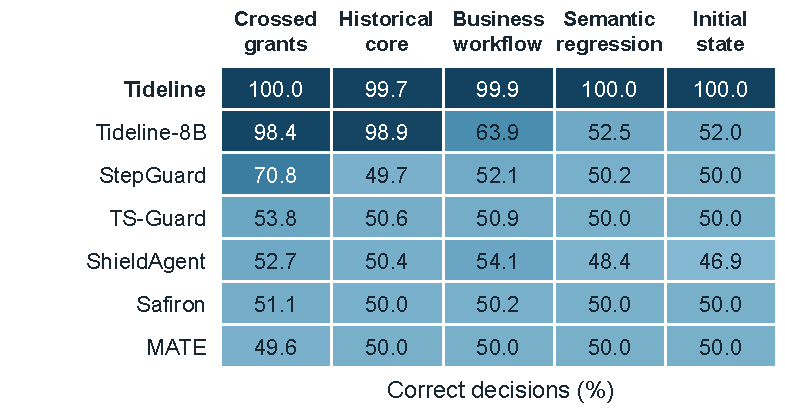
\includegraphics[width=1.0\linewidth]{figures/source_accuracy.pdf}
\caption{Accuracy (percent) by internal source on original tasks, rounded to one decimal. Each cell weights requests within its own source. Table~\ref{tab:strata} gives exact Tideline error counts.}
\Description{Seven reviewer rows and five source columns. The authorization backbone scores higher on the historical sources than on the business and state sets.}
\label{fig:source}
\end{figure}

On the original wording, Tideline-8B scored 98.4\% on the crossed-authorization batches, 63.9\% on the business workflows, and 52.5\% on the quantity-report regression requests (Figure~\ref{fig:source}). With the contextual checks, Tideline answered 2,110 of 2,112 workflow requests and all 1,920 regression requests correctly. Under paraphrase, 21 of 26 errors fell in the workflow batch (seven false blocks and 14 false allows), compared with two false blocks on the original wording. Errors on the reused training requests fell from seven to five.

\paragraph{Contextual routing counts and target-scope head.}
Across the 10,372 original contextual requests, Tideline retained Tideline-8B's default decision 5,596 times and resolved the verdict via the file-effect/permission branch 2,112 times, the snapshot precondition route 2,176 times, the literal-target path head 440 times, and a specialized count-report condition check (reading a first line, last line, or CSV field) 48 times. Across the fixed paraphrases, the corresponding counts were 5,574, 2,112, 2,176, 462, and 48. The literal-target path head applies a two-leaf decision tree fitted on 142 original historical items (124 allow, 18 deny across 23 association groups) from the fitting partition to verify whether a statically traced copy/truncation destination is authorized by the user task.

Table~\ref{tab:axes} counts requests by language and the input changed within each pair. Both wordings use the same programs, workspaces, and reference decisions.

\begin{table}[tb]
\centering\small
\caption{Internal requests in one wording edition. Rows indicate the diagnostic question and columns the language of the candidate.}
\label{tab:axes}
\begin{tabular}{@{}lrrr@{}}\toprule
Changed input & Shell & Python & Total\\\midrule
User request & 2,080 & 2,080 & 4,160\\
Script & 1,288 & 1,288 & 2,576\\
Initial workspace state & 1,818 & 1,818 & 3,636\\\midrule
Total & 5,186 & 5,186 & 10,372\\\bottomrule
\end{tabular}
\end{table}

\paragraph{Keeping related items together.}
The development partition grouped requests associated through a source project, quartet, program combination or business workflow. It assigned 4,190 requests to the fitting portion and 6,182 to the remainder. Both wordings of a request shared an assignment. Earlier heads used the original fitting portion. The literal-target head used 142 original historical items in that portion, comprising 124 allow and 18 deny examples from 23 association groups. Separately, the 2,112 business-workflow items supported file-level modeling. Fourteen workflows (1,232 items) were used for training, four (352) for development and six (528) for testing in that study. The partitions shared construction templates. Both wording editions informed subsequent diagnosis and selection.

\paragraph{Counting groups.}
For a group $G$ of two or four requests, complete correctness is $\prod_{i\in G}\mathbf{1}[\hat y_i=y_i]$. Average this indicator over groups of the same kind and wording. For item accuracy, instead sum the individual indicators and divide by the number of requests. The two averages need different denominators. For example, a four-cell group with three correct decisions contributes 75\% to its item score and zero to its complete-group score. Table~\ref{tab:removal} also gives the item-level counts of false blocks and false allows.

\section{Command Labels, Fitting and Paired Uncertainty}
\label{app:external}
\paragraph{Which rows enter scoring?}
The three sources supplied 4,407 identifiers corresponding to 4,404 distinct visible inputs. Reviewers assessed each distinct input twice. Mapping the votes back to identifiers gives 3,186 consensus allows, 443 consensus holds, 369 pairs of insufficient-evidence votes and 409 disagreements. The first two counts sum to 3,629. Three of those rows lacked an upstream binary label. Restricting scoring to the original binary-labeled population therefore leaves 3,626 consensus rows. The remaining 777 of 4,403 scored rows use the upstream binary label. Across the scored rows, 245 labels changed from allow to hold and 28 from hold to allow. The 4,404 distinct visible inputs used for review are a different population from the 4,403 scored identifiers.

\begin{table}[tb]
\centering\small
\caption{Reconciliation by external source in the main run. The last two columns count errors on scored identifiers.}
\label{tab:sources}
\begin{tabular}{@{}lrrrr@{}}\toprule
Source & Received & Scored & False blocks & False allows\\\midrule
ShellRisk-Bench & 4,194 & 4,194 & 72 & 50\\
shell-guard-bench & 201 & 197 & 8 & 8\\
agent-policy-bench & 12 & 12 & 0 & 2\\\midrule
Total & 4,407 & 4,403 & 80 & 60\\\bottomrule
\end{tabular}
\end{table}

\paragraph{Template groups.}
For template comparison, the normalizer substitutes a common marker for quoted spans, matched paths, selected filename forms and numbers, then normalizes whitespace. Commands sharing the resulting string have one group identity. The fitting partition covers 1,428 such templates. The held-out portion covers another 2,263. Near-equivalent commands that the normalization maps to different strings can appear across the partition. This definition also explains the distinction between a visible-input duplicate, which includes its working directory, and a shared template, which groups command text at a coarser resolution.

\paragraph{Fitting the score.}
The lexical estimator uses sublinear TF--IDF character features of length two to five. It requires a feature in at least two documents and retains up to 70,000 features. The logistic classifier uses balanced class weights and $C=6$. For tabular features, the fit retains columns nonzero in at least three training rows. The randomized forest uses 220 trees, feature fraction .55 and minimum leaf size two. The boosted model uses 125 stages, learning rate .05, depth two and minimum leaf size seven. Each fold fits these transformations and estimators using its own training rows.

For a feature set, the grid assigns lexical weight in $\{.05,.12,.20\}$ and randomized-tree weight in $\{.25,.45,.65\}$, with the remainder assigned to boosting. The threshold ranges from .220 through .660 in increments of .005. On out-of-fold predictions the search first minimizes the larger of the two error counts, then their sum, then the absolute distance of the threshold from .5. Across feature sets the first two criteria select the final configuration. The held-out labels do not enter this grid search.

\paragraph{Blind consensus review and calibration details.}
Figure~\ref{fig:label_review} shows pairwise agreement across the three randomized blocks of 1,468 unique visible commands (Cohen's $\kappa$ = 0.741, 0.752, and 0.811 for A/B, A/C, and B/C); most disagreements involved one reviewer selecting insufficient evidence rather than opposite binary votes (only 3, 3, and 5 direct flips across the three blocks). For the command-only fallback, the selected five-fold cross-validated score combines the lexical ($p_L$), randomized-tree ($p_T$), and boosted-tree ($p_B$) probabilities via $s = 0.20p_L + 0.65p_T + 0.15p_B$, issuing a hold when $s \ge 0.435$. Figure~\ref{fig:calibration} compares five-fold out-of-fold errors across all eight candidate feature sets on the 1,750 fitting items (69 out-of-fold errors for the selected configuration; 4 errors after refitting on all 1,750 items; 136 errors on the 2,653-item template holdout).

\begin{figure}[tb]
\centering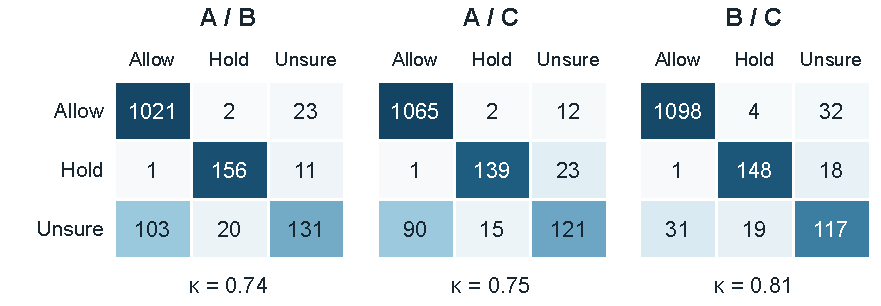
\includegraphics[width=\linewidth]{figures/label_review.pdf}
\caption{Paired blind judgments on external standalone commands before binary scoring (1,468 unique visible inputs per block).}
\Description{Three three-by-three matrices showing that most off-diagonal entries involve an unsure vote rather than opposite binary verdicts.}
\label{fig:label_review}
\end{figure}

\begin{figure}[tb]
\centering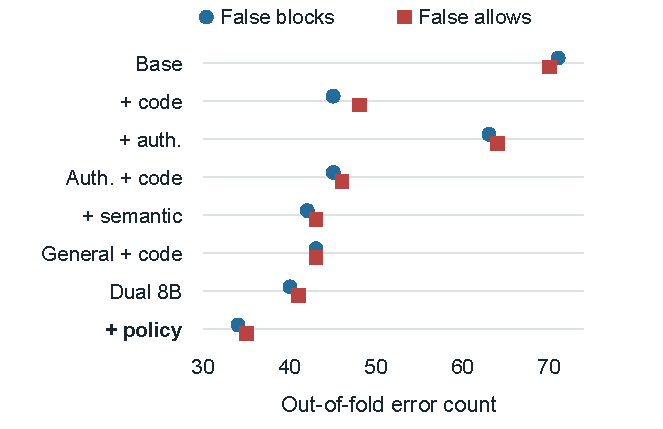
\includegraphics[width=.94\linewidth]{figures/calibration.pdf}
\caption{Five-fold out-of-fold errors across eight candidate feature sets on the 1,750 fitting commands. Dots count false blocks and squares count false allows.}
\Description{Static features yield 71 false blocks and 70 false allows; adding code encoders, language models, and operations-policy features reduces errors to 34 and 35.}
\label{fig:calibration}
\end{figure}

\paragraph{Encoder comparisons.}
For each held-out request, record whether the full and reduced configurations agree with its binary label. Count a correction when the reduced model alone is correct and a new error when the full model alone is correct. Figure~\ref{fig:turnover} reports individual decision turnover: removing the general Qwen3-8B, risk CodeBERT, and joint CodeBERT encoders corrected 22, 30, and 33 errors while introducing 38, 38, and 36 new errors, respectively. The accuracy difference in percentage points is $100$ times corrections minus new errors, divided by 2,653, with the subtraction performed before division. For uncertainty, sample 2,263 template groups with replacement and include every row in each sampled group with its multiplicity. Compute the difference on the resulting row count, which can vary across draws. Each configuration uses the same sampled groups as its comparator. We used 10,000 draws with seed 20261121. The individual intervals are the 2.5th and 97.5th percentiles. The simultaneous comparisons use Bonferroni-adjusted percentile tails of $2.5/3$ percent each.

\begin{figure}[tb]
\centering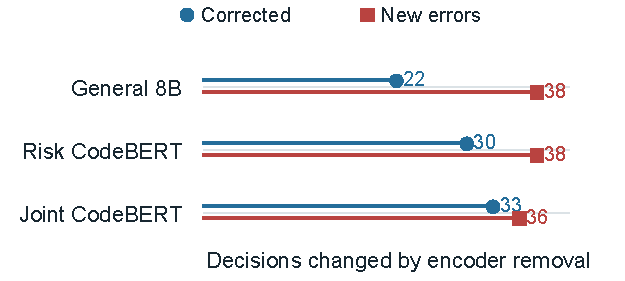
\includegraphics[width=\linewidth]{figures/turnover.pdf}
\caption{Individual decision turnover on the 2,653-item template holdout after retraining without one encoder.}
\Description{Removing the general, risk, and joint encoders corrects 22, 30, and 33 errors while introducing 38, 38, and 36 new errors.}
\label{fig:turnover}
\end{figure}

\section{Public Reviewer Adapters, API Protocol, and Resource Measurement}
\label{app:resources}
For each contextual request, the adapter supplies a user task, a shell tool with command and working directory, local code, and state containing the project documentation and supporting files. The requesting agent's subsequent messages and the evaluator's observations are unavailable at this point. StepGuard and MATE use their corresponding prompt builders and verdict parsers. The TS-Guard adapter supplies three fields for the task, action and environment. It maps a warning or a maximum-risk score to hold. The Safiron adapter serializes the candidate as a single agent action with environment information. ShieldAgent receives the available evidence and the trace prefix ending at the proposed tool call. An invalid verdict counts as an incorrect item in the accuracy denominator. Safiron produced one such verdict among the 10,372 original internal requests.

\subsection{Offline API Baseline Protocol and Parsing Reconciliation}
\label{app:api-protocol}
Both API baselines operated on the exact same frozen visible inputs as the checkpoint adapters across all 25,151 requests (10,372 original internal, 10,372 fixed paraphrase, and 4,407 external, of which 4,403 carry binary scoring labels). Codex Auto Review invoked request model ID \texttt{codex-auto-review} through the Responses API, and Sonnet~5 (low) invoked \texttt{claude-sonnet-5} through the Messages API (\texttt{thinking.type=\allowbreak adaptive}, \texttt{output\_config.effort=\allowbreak low}, \texttt{max\_tokens=\allowbreak 4096}). Both were routed through a third-party API gateway whose responses returned matching model IDs. Neither run recreated native client reviewer prompts or executed interactive agent sessions, and no response was resampled on correctness or format.

Many Sonnet~5 (low) responses included explanatory prose alongside a JSON verdict, causing whole-string strict JSON parsing to fail on 7,488 of 25,151 responses. Under the unique explicit-decision extraction rule, surrounding text is accepted only when all explicit decision values in parsed JSON objects agree on \texttt{allow} or \texttt{deny}. This rule recovers 7,410 format-only responses while keeping 78 invalid responses unrecovered: 52 with conflicting or unknown decisions, 17 with no explicit JSON decision, and 9 incomplete responses. Invalid responses are counted as incorrect rather than remapped to denials. Table~\ref{tab:api-parsing} summarizes these counts by evaluation group. Applying the identical explicit-decision rule to all 25,151 Codex Auto Review responses leaves every decision unchanged (0 invalid).

\begin{table}[tb]
\centering\small
\setlength{\tabcolsep}{4pt}
\caption{Sonnet~5 (low) invalid responses under unique explicit-decision extraction across all 25,151 requests (7,488 whole-string strict parse failures, 7,410 recovered, 78 remaining invalid: 52 conflicting/unknown, 17 missing decision, 9 incomplete). Codex Auto Review had 0 invalid responses under the same rule.}
\label{tab:api-parsing}
\begin{tabular}{@{}lrr@{}}\toprule
Evaluation group & Requests & Invalid\\\midrule
Internal, original wording & 10,372 & 40\\
Internal, fixed paraphrase & 10,372 & 29\\
ShellRisk-Bench (full / held) & 4,194 / 2,511 & 7 / 2\\
shell-guard-bench (full / held) & 197 / 135 & 2 / 2\\
agent-policy-bench (full / held) & 12 / 7 & 0 / 0\\\midrule
Total scored (+4 unscored) & 25,147 (+4) & 78\\\bottomrule
\end{tabular}
\end{table}

The resource measurement starts after model initialization and warm-up (Figure~\ref{fig:cost}). Each fresh process warms up on 32 fitting requests, synchronizes the devices and resets the peak-allocation counters. Timing covers successive batches of eight, including the final partial batch. The reported mean time per item divides the sum of synchronized batch times by the number of requests. Peak allocation sums the PyTorch device peaks within that process. It measures model-side allocation across the cards and excludes memory outside the allocator. Dividing this quantity by the number of cards would answer a different hardware question. In a reversed-order verification on a second pair of RTX~5090 cards over 192 held-out requests, full Tideline took 198.3 and 198.8~ms/item while the single-GPU variant without general Qwen3-8B took 156.9~ms/item in both runs.

\begin{figure}[tb]
\centering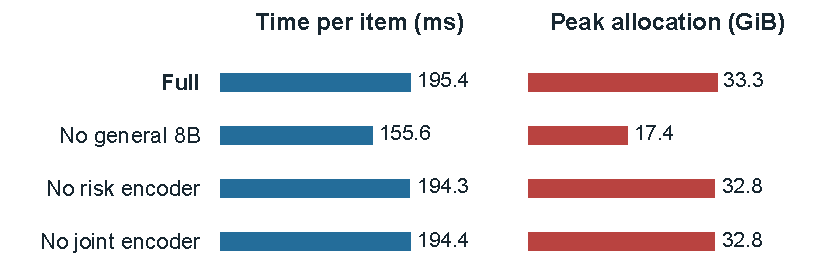
\includegraphics[width=\linewidth]{figures/resource_cost.pdf}
\caption{Amortized processing time per request and peak allocated GPU memory across command-encoder ablations on the 2,653-item template holdout.}
\Description{Removing the general 8B encoder yields the largest decrease in both latency per item and summed GPU memory.}
\label{fig:cost}
\end{figure}

\section{Continual Update Protocol, Transfer, and Policy Decoupling}\label{app:update-transfer}
Figure~\ref{fig:continual-updates} illustrates how our continual-learning pipeline constructs single-factor paired update cases verified by before-and-after workspace snapshots while keeping Tideline-8B's 8B encoder frozen~\cite{rolnickreplay,raasfig}. Each illustrative grid isolates one factor under active host policy rules. In the tool-update grid, versions v2-R and v2-A add department~A index writes to the requested report, so a report-only request permits v1 alone. In the task-grant grid, holding v2-A fixed, naming department~A authorizes the append while naming department~B withholds it. In the warehouse-stage grid, opening, sealing, and reopening a count sheet flips permission for the same inventory request.

\begin{figure*}[t]
\centering
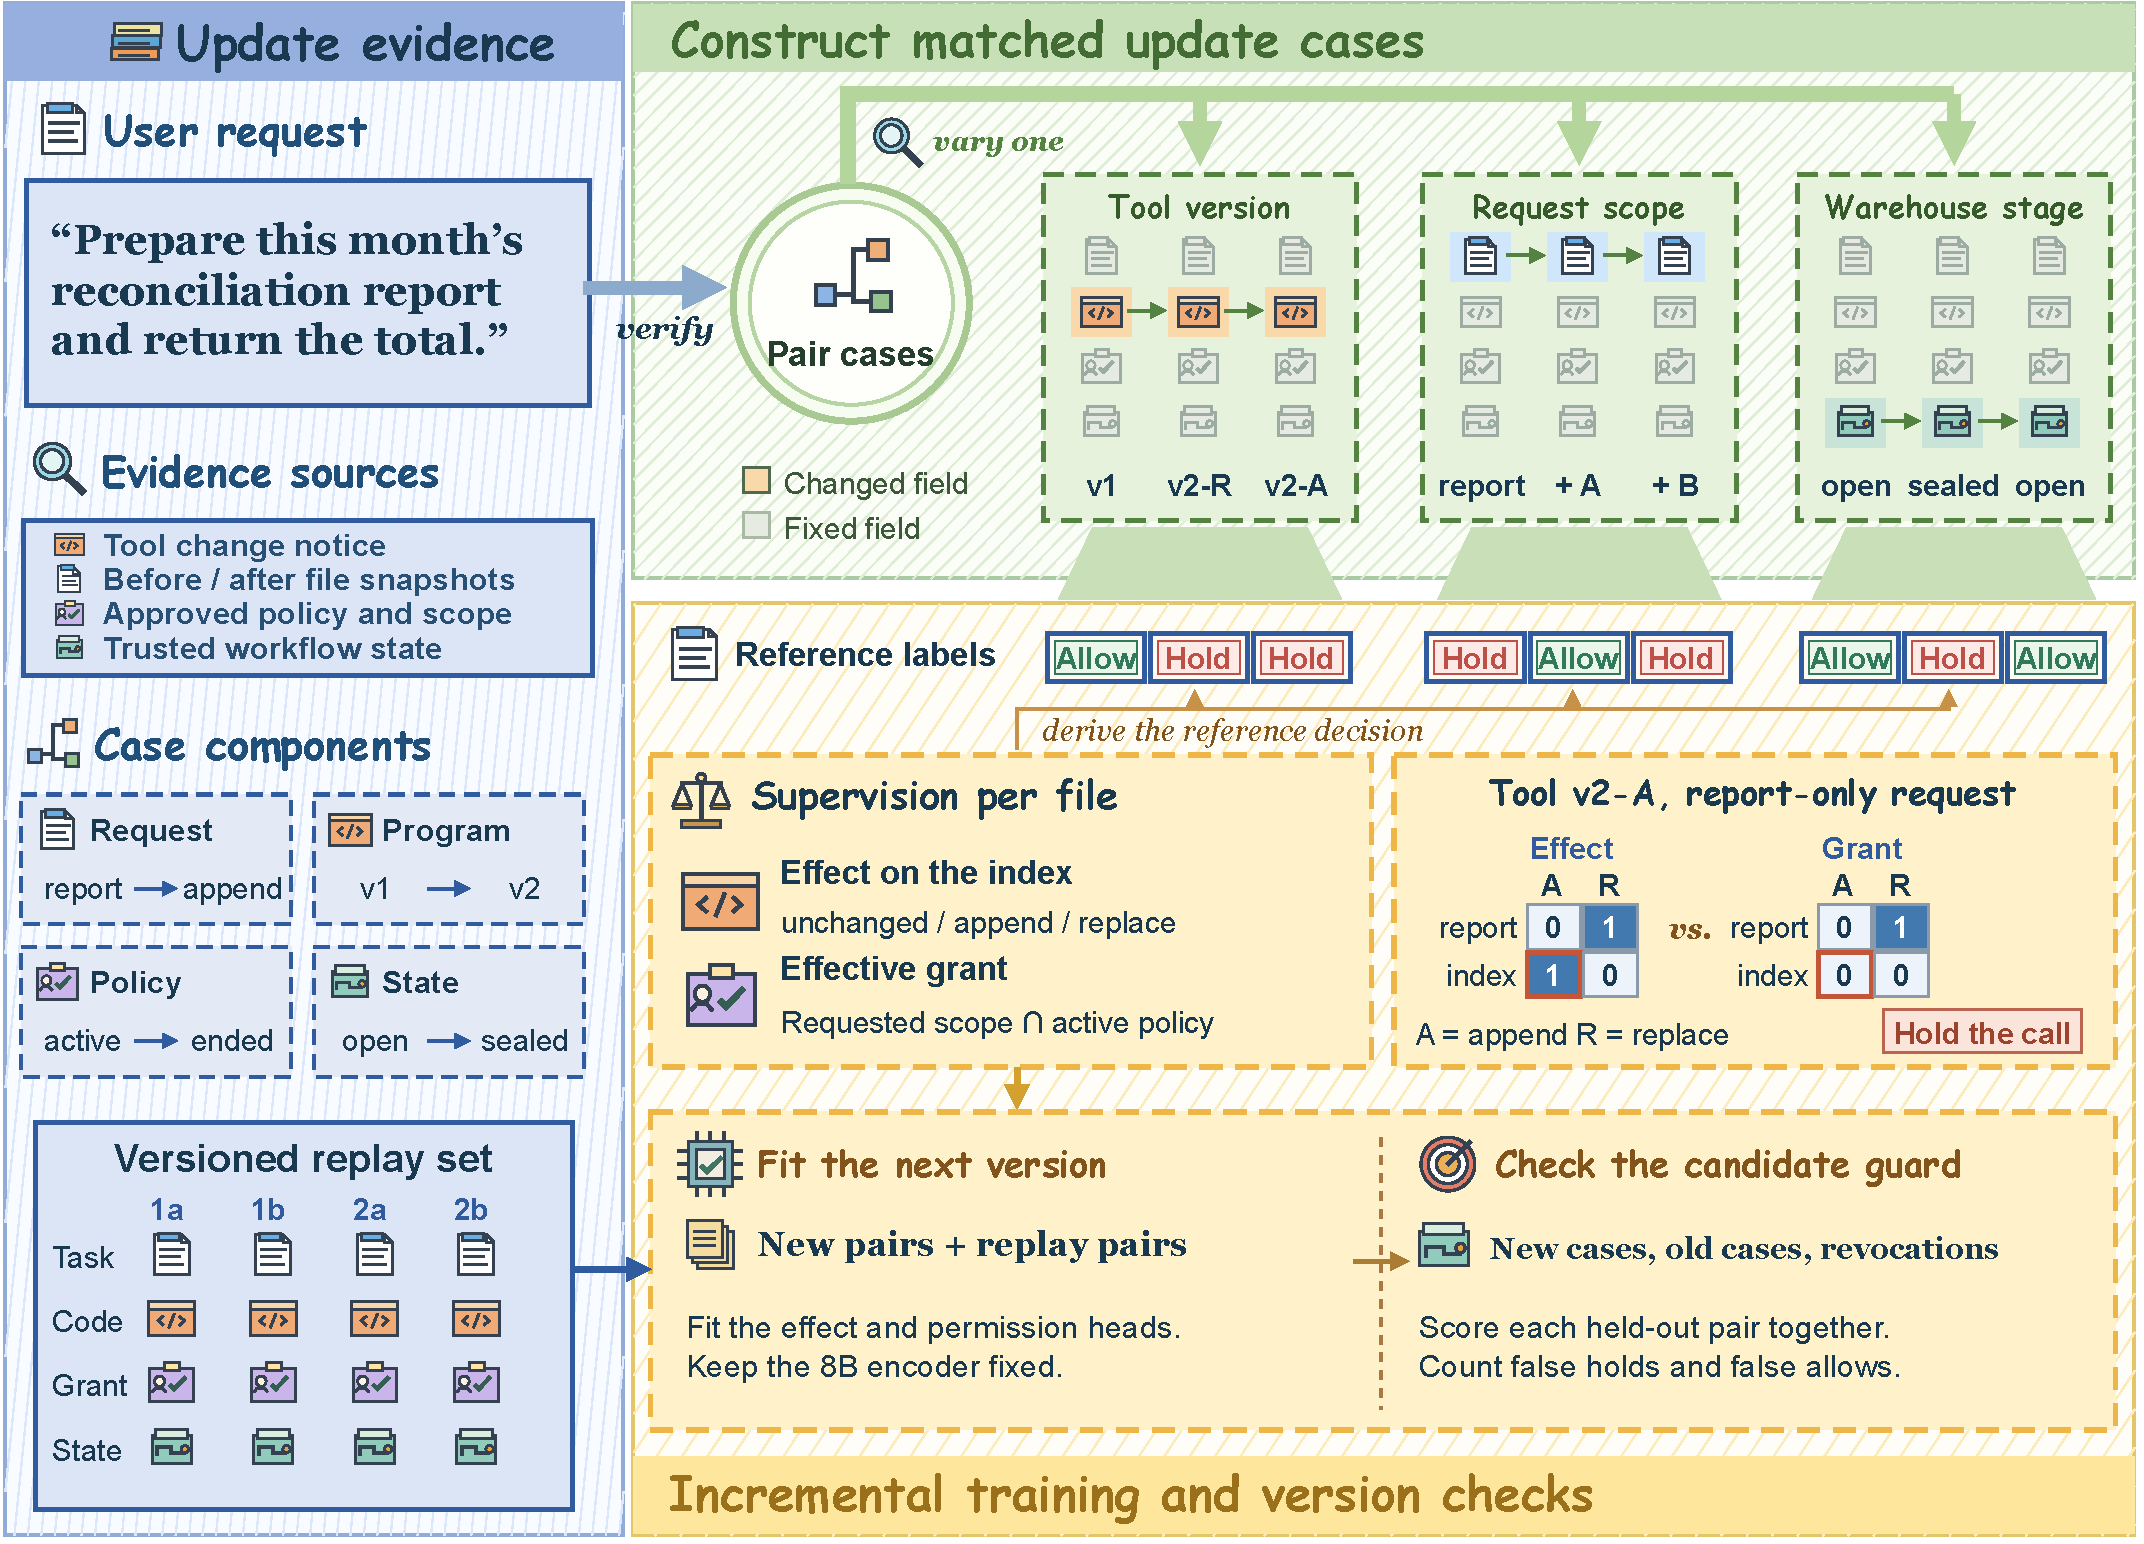
\includegraphics[width=\linewidth]{figures/continual_updates.pdf}
\caption{Versioned continual-learning protocol for Tideline. Paired cases illustrate expected decisions that isolate tool updates, task grants, and workflow states under snapshot verification and experience replay~\cite{rolnickreplay}. Panel layout adapted from Yang et al.~\cite{raasfig}, Fig.~2.}
\Description{Single-factor paired examples compare tool behavior, user requests, and workflow states with append and replace indicators. In the tool v2-A worked example, the matrices record verified file changes (report replacement and index append) against an effective grant covering report replacement only, yielding a hold target. The update loop initializes both file readouts from the prior version, keeps the 8B encoder fixed, replays policy-versioned pairs after rechecking revoked permissions, and retains the active policy on model rollback.}
\label{fig:continual-updates}
\end{figure*}

Separate from the illustrative grids, we measured a sequential update across 60 tool-version cases, 60 authorization cases, and 28 warehouse cases, evaluated on 204 held-out Shell and Python calls (96 authorized and 108 requiring a hold). Prior to updating, the frozen readouts missed 18 unauthorized calls and issued 62 false holds. With experience replay at seed~41, missed holds dropped to 0/108 and complete three-call tool-version groups rose from 7/12 to 9/12, while false holds shifted from 62 to 81, opposite-label pairs shifted from 28/120 to 24/120, and unseen request-scope and warehouse-stage groups remained at 0/12. Tracking both missed holds and false holds in that measurement established the two-sided evaluation protocol used in Section~\ref{sec:rq4}.

A rollback test held the current policy fixed after revoking a delegate's right to append to an index. The updated heads held all 12 affected calls. Restoring the original weights allowed two calls to change the index despite the revocation. An additional check held a call when a grant had been withdrawn and static analysis could not establish its complete effects. It prevented both writes and also held all 12 report-only controls, eight of which the rolled-back reviewer had allowed.

We next took cancellation actions for 20 retail orders and 13 airline reservations from the $\tau$-bench test trajectories~\cite{taubench}. The guard saw the proposed change as a replacement of the principal record, with eligibility supplied from the published policy. On copies of the upstream databases, the seed~41 replay model blocked all 33 ineligible cancellations and ran all 33 refund inquiries as well as the 33 confirmed cancellations. Frozen and current-batch heads made the same decisions. The 33/33 eligibility pairs and 0/33 consent pairs motivated a separate transfer test on new operations.

Starting from the same seed~41 replay checkpoint, we supplied 16 cancellation pairs from distinct orders in the official retail training split. Within each pair only the user's final confirmation changed. We tested on 17 retail address changes and five airline baggage changes from the official test split. The upstream tools verified that each proposed update changed the intended record in the initial database. Each object supplied two pairs that shared a confirmed request, one paired with an inquiry and the other with an explicit refusal. The experiment uses published actions, arguments, and objects together with constructed confirmation exchanges and single-action labels.

\begin{table}[!ht]
\centering\small
\caption{Fully correct pairs after fitting 16 retail cancellation pairs. Entries list counts for seeds 41, 73, and 109 in order. Each column gives its denominator. All updates start from the same parent.}
\label{tab:continual-transfer}
\begin{tabular}{@{}lccc@{}}\toprule
Update regime & Retail (/34) & Airline (/10) & Prior file (/120)\\\midrule
Common parent (seed 41) & 14 & 0 & 24\\
Current batch only & 28, 34, 24 & 0, 0, 0 & 0, 0, 0\\
Paired replay & 34, 19, 34 & 0, 8, 0 & 24, 24, 24\\\bottomrule
\end{tabular}
\end{table}

Table~\ref{tab:continual-transfer} shows that cancellation supervision improved address-change consent decisions at all three seeds, and replay retained the parent's 24 correct file pairs while current-batch updates retained zero. Across the five airline objects, replay yielded 0, 8, and 0 correct pairs out of 10. Seed~73 also missed 15 retail requests that required a hold. With seed~41 and replay, direct execution through the gate applied all 17 confirmed address changes and blocked the other 34 address requests. The same gate blocked all 15 baggage requests, including the five authorized updates.

For the OpenFGA study in Section~\ref{sec:rq4}, we enumerated all 1,603 boolean Check assertions from 54 test stores across 40 parent directories at commit \texttt{6802b4d8}~\cite{openfgastores}, normalizing to 51 distinct policy models. Running OpenFGA CLI~v0.9.0 reproduced 1,603/1,603 authored labels. Deduplicating identical policy text, effective tuples, requests, and contexts left 1,548 distinct public checks (971 allowed, 577 denied, and 62 with extra context), all 1,548/1,548 reproduced from normalized inputs. Pairing each public check with six local Shell and Python variants (report-only, log-append, log-replace) produced 9,288 derived local requests (4,250 requiring a hold and 5,038 authorized) spanning 12 source implementations, two equivalent condition phrasings, and 72 distinct encoded effect views.

Pre-update evaluations across all 9,288 derived requests clarify the architectural division between host policy evaluation and file-effect readouts. Reading host permission status alone reached 6,192/9,288 with 1,942 missed holds and 1,154 false holds (0/1,548 all-six checks), whereas static parsing that holds unresolved writes reached 4,250/9,288 with 0 missed holds and 5,038 false holds (0/1,548 all-six checks). Pre-update replay readouts scored 4,284/9,288 with 7 missed holds and 4,997 false holds (1/1,548 all-six), and disabling the condition evaluator gave 4,279/9,288. Presenting raw OpenFGA policy text and tuples directly to the file branch without host evaluation on the 1,548 append checks (max 1,043 tokens, zero truncation) triggered the condition evaluator zero times and caused the pre-update readouts to hold all 1,548 items (577/1,548 correct, versus 652/1,548 for an earlier readout checkpoint). Delegating authorization graph evaluation to OpenFGA while restricting readout learning to file effects and host-state checks avoids forcing the 8B file heads to solve external policy graphs from text.

In the four-window streaming update (34 policies split 9, 9, 8, and 8, totaling 1,064 checks and 6,384 pre-feedback items under seed~41), 8 checks per window (32 checks total) were selected by deterministic stable-ID ordering after excluding checks whose joint encoded inputs reoccurred in another window or the holdout, without using test labels. Pre-feedback accuracy across all four windows was 2,954/6,384 for frozen readouts (5 missed, 3,425 false holds, 1/1,064 all-six), 4,647/6,384 for current-batch fitting (0 missed, 1,737 false holds, 218/1,064 all-six), 4,333/6,384 for paired replay (0 missed, 2,051 false holds, 266/1,064 all-six), and 5,600/6,384 for exact-verdict memory (0 missed, 784 false holds, 823/1,064 all-six). Because exact-verdict binary memory covered all 24 observed keys in the shared-style update, we ran the reciprocal crossed-style evaluation as a follow-up diagnostic. Each fold started independently from the same pre-update checkpoint, received 32 checks (192 feedback requests) in its own style across four windows at seed~41, and held out scripts absent from that fold's new feedback (though those language constructs had appeared in earlier training of the initial checkpoint). Each source check yielded all six variants within a single test fold, and pooling the disjoint test items from both folds gave the 2,904 held-out decisions. Fold~0 trained on \texttt{printf} and \texttt{open} and tested on \texttt{echo} and \texttt{Path.open} (1,476 requests across 246 checks), lifting item accuracy from 692 (frozen and memory) to 1,045 (current) and 1,249 (replay), with complete all-six checks rising from 0 to 43 and 58 out of 246. Fold~1 reversed the styles (1,428 requests across 238 checks), raising accuracy from 638 (frozen and memory) to 1,032 (current) and 1,188 (replay), while all 238 Python report-only items received false holds when \texttt{open} was held out. The shared-style experiment scored each entire window before feedback. In each crossed-style fold, we scored the 48 selected requests in each window before updating on them. For live gating we selected the first check in stable ID order for each OpenFGA verdict present in each source file. This yielded 33 checks, for which we gated all six variants. Live execution gates evaluated those 198 requests (100 authorized, 98 prohibited): under shared-style updates, the replay gate blocked 98/98 prohibited calls and ran 93/100 authorized requests (coinciding with the offline batch on all 198 items), whereas under the crossed-style diagnostic the two corresponding fold models blocked 98/98 prohibited calls and ran 71/100 authorized requests (with two of the 198 individual replay judgments differing from the offline batch). Finally, on retention checks after the shared-style update, frozen, current-batch, and replay readouts answered 416, 412, and 404 of 528 held-out business workflow requests (58, 72, and 69 missed holds), and solved 100, 68, and 90 of 144 earlier condition-flipping pairs (8, 32, and 6 missed holds).
